%!TEX root = main.tex
\chapter{Análisis y conclusiones}
En este capítulo se presentan los resultados obtenidos en el desarrollo de esta
memoria.
En la sección~\ref{sec:datos} se muestra información y estadísticas de los datos
analizados como son las fechas, los tipos de consultas, los \emph{endpoint} más
utilizados y otra información relevante del proyecto Bio2RDF.

La sección~\ref{sec:res} presenta los resultados obtenidos tanto de la
extracción y creación del grafo RDF como del cálculo de su centralidad. Con
estos datos se hacen los análisis y las comparaciones pertinentes.

Por último, en la sección~\ref{sec:con}, se enuncian las conclusiones generales
obtenidas junto a una comparación de ellas con lo que se espera del proyecto
Bio2RDF. Además se evidencian los problemas detectados y se genera una lista de
posibles mejoras y trabajo futuro con respecto a este tema.


\section{Datos analizados}\label{sec:datos}
Para el análisis llevado a cabo en este trabajo se dispuso de 12Gb de consultas
almacenadas en 57.016 archivos de registros obtenidos del proyecto Bio2RDF.
Cada linea de un archivo de registro almacena una consulta y metadatos 
relacionados a ella en forma de diccionario \tt{json}. En esta sección se
analizarán estos datos.

Con respecto a la fecha, las consultas fueron efectuadas entre el 05 de mayo del
2013 hasta el 18 de septiembre del 2015.
La figura~\ref{fig:dates} muestra una gráfica de la distribución de consultas
realizadas al proyecto en este periodo.
Para el análisis debemos tener en cuenta que los datos del mes inicial y final
se registraron completamente.

\begin{figure}[ht]
  \begin{tikzpicture}
    \begin{axis}[
        xlabel=Fecha (año-mes), ylabel=Número de consultas,
        xticklabel style={rotate=90,anchor=near xticklabel},
        width=\textwidth,height=6cm,compat=1.9,
        date coordinates in=x,date ZERO=2013-05-01,
        ymin=0,ymax=1500000, xticklabel=\year-\month,
        xmin=2013-04-01,xmax=2015-10-01]
      \addplot table [x=date,y=value,col sep=comma]{data/mdates.csv};
    \end{axis}
  \end{tikzpicture}
  \caption{Fechas de las consultas.}\label{fig:dates}
\end{figure}

Los registros disponen de una total de 12.881.518 consultas hechas por 9.818 IPs
diferentes, las cuales realizaron entre 1 y 2.831.912 peticiones cada una.

En la figura~\ref{fig:ips} se muestra la cantidad de IPs que realizan hasta
cierto número de consultas.
Como podemos ver en ella, la mayoría de las IPs efectuó entre 1 y 100 consultas,
pero su aporte al total es bajo (menos de 1\%), de hecho, las 23 IPs con mayor
cantidad de consultas (más de $10^5$) aportan cerca del 80\% del total, el
detalle de estas IPs puede ser visto en la tabla~\ref{tab:ips}.

\begin{figure}[ht]
  \begin{tikzpicture}
    \begin{axis}[ybar, ymin=0, ymax=4500,
        xlabel=Número de consultas, ylabel=Número de IPs,compat=1.9,
        width=\textwidth,height=6cm,
        xtick=data,
        xticklabels={{$1$},{$10$},{$10^2$},{$10^3$},{$10^4$},{$10^5$},{$10^6$},{$10^7$}},
        nodes near coords,
        nodes near coords align={vertical}]
    \addplot table [x expr=\coordindex,y=value,col sep=comma]{data/ip.csv};
    \end{axis}
  \end{tikzpicture}
  \caption{Cantidad de consultas por IP.}\label{fig:ips}
\end{figure}

\begin{table}[ht]
  \centering
  \begin{tabular}{|r|l|l|l|} \hline
    \bf{Consultas} & \bf{IP} & \bf{Pais} & \bf{Instituación} \\\hline
    121646  & 150.214.40.112  & España         
                   & Centro Informatico Cientifico de Andalucia\\\hline
    129006  & 37.6.165.5      & Grecia         
                   & Desconocido\\\hline
    134178  & 79.107.219.216  & Grecia         
                   & Desconocido\\\hline
    141036  & 134.160.214.42  & Japón          
                   & RIKEN\\\hline
    143496  & 134.117.221.16  & Canadá         
                   & Carleton University\\\hline
    150236  & 155.185.49.66   & Italia         
                   %& Universita Degli Studi Di Modena E Reggio Emilia\\\hline
                   & Degli Studi Di Modena E Reggio Emilia\\\hline
    153794  & 134.117.108.151 & Canadá         
                   & Carleton University\\\hline
    166286  & 24.130.52.25    & EEUU 
                   & Desconocido\\\hline
    167895  & 134.117.108.111 & Canadá         
                   & Carleton University\\\hline
    217148  & 134.117.108.158 & Canadá         
                   & Carleton University\\\hline
    229289  & 173.178.48.100  & Canadá         
                   & Desconocido\\\hline
    232020  & 140.203.154.5   & Irlanda        
                   & National University of Ireland Galway\\\hline
    233677  & 159.90.11.58    & Venezuela      
                   & Universidad Simón Bolívar\\\hline
    238541  & 134.117.108.159 & Canadá         
                   & Carleton University\\\hline
    251789  & 146.155.115.75  & Chile          
                   & Pontificia Universidad Católica de Chile\\\hline
    259143  & 140.203.154.6   & Irlanda        
                   & National University of Ireland Galway\\\hline
    304598  & 133.11.132.151  & Japón          
                   & University of Tokyo\\\hline
    342553  & 140.203.154.11  & Irlanda        
                   & National University of Ireland Galway\\\hline
    478989  & 129.26.128.185  & Alemania       
                   & Fraunhofer-Gesellschaft\\\hline
    801417  & 129.26.131.1    & Alemania       
                   & Fraunhofer-Gesellschaft\\\hline
    1130035 & 134.117.221.14  & Canadá         
                   & Carleton University\\\hline
    1391974 & 171.65.32.83    & EEUU 
                   & Stanford University\\\hline
    2831912 & 132.203.117.5   & Canadá         
                   & Universite Laval\\\hline
  \end{tabular}
  \caption{IPs con más consultas.}\label{tab:ips}
\end{table}

En la tabla~\ref{tab:ips} además podemos notar como la mayoría de las
instituciones a las cuales pertenecen las IPs son universidades o centros de
investigación.

Este fenómeno era de esperar ya que, aunque los datos sean públicos, la
naturaleza de ellos los hace útiles sólo para el publico especializado, ya sea
para la investigación biológica o en la relacionada a la informática.

En la figura~\ref{fig:size} se presenta una gráfica de la cantidad de consultas
registradas y el peso de la respuesta correspondiente. Estas respuestas van
desde el rango de los kilobytes (entre $2^{10}$ y $2^{19}$), pasando por los
megabutes (entre $2^{20}$ y $2^{29}$) y llegando incluso a los gigabytes (entre
$2^{30}$ y  $2^{39}$).
Como podemos ver en ella, la mayor cantidad de consultas tiene retornos de unos
pocos kilobytes o menos.
Generalmente esto corresponde a tablas con pocas filas (o ninguna),
identificadores de retorno vacío (\tt{\# Empty NT}) o resultados de operaciones
más complejas (como calcular promedios, contar recursos según ciertos filtros,
etc).

La mayor concentración se encuentra en el rango de los kilobytes y al principio
de los megabytes.
Pocas consultas retornan más de un gigabyte de datos y posiblemente
corresponden a consultas como la de la figura~\ref{fig:exbigq} y similares que
retornan toda la base de datos.

\begin{figure}[ht]
  \begin{tikzpicture}
    \begin{axis}[
        xlabel=Tamaño de la consulta (en bytes), ylabel=Número de consultas,
        width=\textwidth,height=6cm,compat=1.9,
        xticklabel={2\textsuperscript{\pgfmathprintnumber{\tick}}},
        ymode=log,
        xmin=8,xmax=32]
      \addplot table [x=exp,y=n,col sep=comma]{data/size.csv};
    \end{axis}
  \end{tikzpicture}
  \caption{Tamaño de las consultas.}\label{fig:size}
\end{figure}

Como se explica en la sección~\ref{d:emc} los registros almacenan el tipo de
consulta hecha al servidor en los atributos \tt{DESCRIBE}, \tt{ASK},
\tt{CONSTRUCT} y \tt{SELECT}. Generalmente se marca con un $1$ cuando la
consulta es de ese tipo y con un $0$ en caso contrario pero existen dos casos
particulares.
Si la consulta presenta un error todos los atributos se marcarán como una cadena
de caracteres vacía, y si no se puede determinar el tipo, todos los atributos
serán 0. Si sucede lo último diremos que la consulta es de tipo ``desconocido''.

\begin{figure}[ht]
  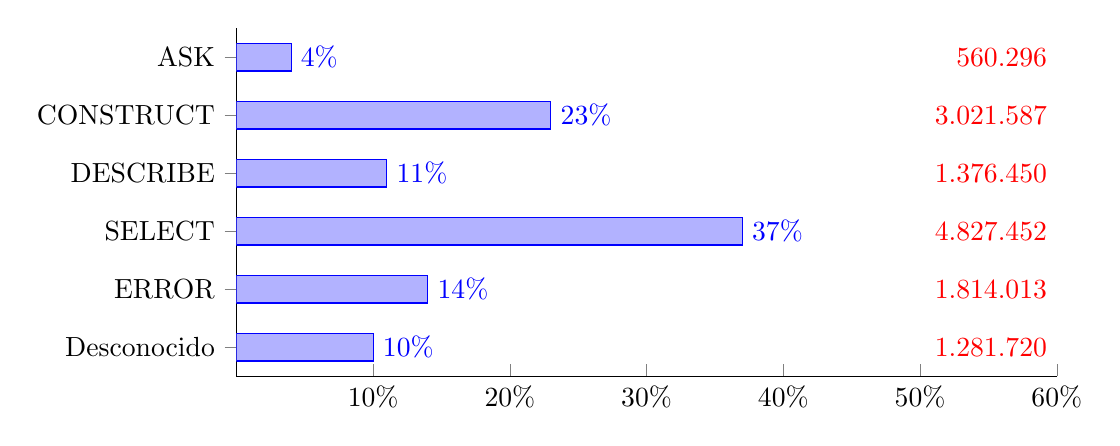
\begin{tikzpicture}
    \begin{axis}[axis lines*=left, xbar, width=12cm, height=6cm, xlabel={},
      symbolic y coords={Desconocido, ERROR, SELECT, DESCRIBE, CONSTRUCT, ASK },
      ytick=data, xmin=0, xmax=0.6, nodes near coords,
      nodes near coords align={horizontal},xtick={0.1, 0.2, 0.3, 0.4, 0.5, 0.6},
      xticklabel={\pgfmathparse{\tick*100}\pgfmathprintnumber{\pgfmathresult}\%},
      point meta={x*100},
      nodes near coords={\pgfmathprintnumber\pgfplotspointmeta\%},
      nodes near coords align={horizontal}]
      \addplot coordinates
      {(0.37,SELECT) (0.23,CONSTRUCT) (0.11,DESCRIBE)
       (0.04,ASK) (0.10,Desconocido) (0.14,ERROR)};

      \node[red,left] at (axis cs:0.6,SELECT)      {4.827.452};
      \node[red,left] at (axis cs:0.6,CONSTRUCT)   {3.021.587};
      \node[red,left] at (axis cs:0.6,ASK)         {560.296};
      \node[red,left] at (axis cs:0.6,ERROR)       {1.814.013};
      \node[red,left] at (axis cs:0.6,DESCRIBE)    {1.376.450};
      \node[red,left] at (axis cs:0.6,Desconocido) {1.281.720};
    \end{axis}
  \end{tikzpicture}
  \caption{Tipo de consultas realizadas.}\label{fig:qtype}
  \vspace{-.2cm}
  \caption*{En rojo el total de consultas por tipo.}
\end{figure}

La figura~\ref{fig:qtype} presenta los tipos de consultas almacenadas en los
registros. Como podemos notar el tipo predominante es \tt{SELECT} seguido de
\tt{CONSTRUCT}. Este es un resultado esperado debido a que la forma más natural
de consultar información a una base de datos es mediante \tt{SELECT} ya que este
retorna la información en una tabla, formato fácil de leer por los humanos.

La aparición de \tt{CONSTRUCT} en segundo lugar denota que gran parte de los
usuarios del proyecto Bio2RDF utilizan los datos directamente como  triples RDF,
posiblemente ya que esto facilita el manejo de los datos por parte de las
computadoras.

Las consultas tipo \tt{ASK} son las menos populares, lo que muestra que
generalmente un usuario prefiere utilizar \tt{SELECT} o \tt{CONSTRUCT} y manejar
un posible retorno vacío, que preguntar si existen los datos primero (aunque
\tt{ASK} sea más rápido, si se requiere obtener los datos después de una
respuesta afirmativa se necesitará una consulta adicional).

\begin{figure}[ht]
  \begin{tikzpicture}
    \begin{axis}[ybar, ymin=0, ymax=38, xtick=data,
        ylabel=Porcentaje del total de consultas,
        flexible xticklabels from table={data/t10endp.csv}{label}{col sep=comma},
        width=\textwidth,height=6cm,compat=1.9,
        xticklabel style={rotate=90,anchor=near xticklabel},
        yticklabel={\pgfmathprintnumber{\tick}\%},
        nodes near coords={\small\pgfmathprintnumber\pgfplotspointmeta\%},
        nodes near coords align={vertical}]
      \addplot table[x expr=\coordindex,y=p]{\tableendp};
    \end{axis}
  \end{tikzpicture}
  \caption{Diez \emph{endpoint} más consultados.}\label{fig:t10endp}
\end{figure}

Por último, la figura~\ref{fig:t10endp} presenta los diez \emph{endpoint} más
consultados en el proyecto Bio2RDF. La barra ``Otros'' agrupa las consultas de
los 35 \emph{endpoint} con menos de $3,5\%$ de consultas cada uno. Cabe destacar
que si bien la consulta se dirige a cierto \emph{endpoint}, los resultados de la
misma pueden ir más allá de este dominio pues una de las ventajas del proyecto
Bio2RDF es la existencia de enlaces entre las diferentes bases de datos.

\section{Resultados obtenidos}\label{sec:res}
En esta sección se presentan los resultados obtenidos de la ejecución de los
programas descritos en el capítulo~\ref{c:desarrollo} junto a pasos 
adicionales y consideraciones para optimizar el proceso.

En la sección~\ref{sec:res:extr} se muestran estadísticas del proceso de
extracción y modificación de consultas, mientras que en la
sección~\ref{sec:res:obt} se hace lo mismo del proceso de obtención de triples.
Por último, en la sección~\ref{sec:res:cent} se presentan los resultados del
calculo de centralidad y datos relacionados a ellos.

\subsection{Extracción y modificación de consultas}\label{sec:res:extr}
Para recrear la porción de la base de datos consultada por los usuarios se
ejecutó el programa descrito en el algoritmo~\ref{alg:extract} sobre todos los
archivos, generando las consultas \tt{CONSTRUCT} correspondientes.

En este proceso 3.750.759 consultas fueron omitidas. Estas corresponden a la
suma de las consultas tipo \tt{ASK}, \tt{DESCRIBE} y \tt{ERROR} de la
figura~\ref{fig:qtype}.

Las 9.130.759 consultas restantes pasaron por el proceso de modificación en el
cual se crearon 9.212.229 consultas y 838 tuvieron errores de procesamiento
(el $0.004\%$).
Como podemos notar se obtuvieron 82.308 consultas más que las procesadas
correctamente, esto es debido a la separación de las clausulas \tt{OPTIONAL} en
consultas diferentes, como es descrito en la sección~\ref{d:emc}.

De las consultas creadas 2.908.304 fueron marcadas como consultas con solo
variables, las cuales fueron guardadas en un archivo diferente para pasar por
filtros adicionales. 
Además, del análisis de las consultas marcadas con errores, se descubrió que
831 de ellas presentan problemas con su codificación ya que fueron guardadas en
formato de código porciento. Otras 6 consultas poseen errores de sintaxis
irrecuperables y solo 1 era valida pero no pudo ser procesada.

\subsection{Obtención de los triples}\label{sec:res:obt}
Para obtener los triples RDF consultados por los usuarios debemos ejecutar las
consultas creadas en el \emph{endpoint} a analizar, en este caso la última
versión de DrugBank, como se describe en la sección~\ref{d:cg}.

Para evitar hacer más consultas de las necesarias se omitieron las consultas
repetidas y, de las consultas con solo variables, se ejecutaron solo aquellas
que poseen algún filtro (\tt{FILTER}). De esta manera se redujo el número de
consultas a 7.014.088.

De este proceso se obtuvieron los siguientes resultados:
\begin{itemize}
  \item
    6640609 consultas tuvieron un retorno vacío (\tt{\#Empty NT}), esto
    corresponde al $94.6\%$ de las consultas analizadas. Todas estas consultas
    poseen datos que no están en DrugBank y por ello no se pueden crear los
    triples requeridos.
  \item
    279892 consultas retornaron datos, esto corresponde a un $4\%$ del total de
    consultas ejecutadas. Este resultado es cercano al $6.6\%$ de consultas que
    DrugBank presenta según la figura~\ref{fig:t10endp}, la diferencia puede ser
    atribuida principalmente a dos factores: el tipo de consulta y aquellas
    consultas que piden datos de más de una base de datos.
  \item
    93587 consultas resultaron en error, esto corresponde a un $1,33\%$, de
    ellas:
    \begin{itemize}
      \item
        86402 son \tt{HTTP Error 500: SPARQL Request Failed}, que significa que
        ocurrió un error interno en el servidor \emph{virtuoso}, esto puede ser
        debido a que se sobrepasó el tiempo máximo de procesamiento o que se
        piden más datos de los permitidos.
      \item 
        7029 son \tt{HTTP Error 400: Bad Request}, que evidencia una consulta
        SPARQL mal formulada, este error es puede ser atribuido a posibles
        errores en el proceso de creación y modificación de las consultas.
      \item
        156 son \tt{HTTP Error 404: File not found}, que es causado cuando un
        recurso que se pide no es encontrado.
    \end{itemize}
\end{itemize}

\subsection{Centralidad}\label{sec:res:cent}
En este punto ya tenemos todos los datos necesarios en un archivo N-Triples. Con
el algoritmo~\ref{alg:convert} estos datos se convierten en un grafo, en este
caso el orden del grafo creado es de 6.364.209, del cual se calcula la
centralidad según el algoritmo~\ref{alg:degree} y el~\ref{alg:bet}.

\subsubsection{Centralidad de grado entrante}
\begin{itemize}
  \item 3.819.971 ($60\%$) obtuvieron una centralidad de 0, de los cuales:
    \begin{itemize}
      \item 3.803.439 ($59,76\%$) son recursos anónimos.
      \item 16.532 ($0,25\%$) son URIs.
    \end{itemize}
  \item 2.544.238 ($39,97\%$) tienen centralidad entre 1 y 1.453.738, de los cuales:
    \begin{itemize}
      \item 1.377.801 ($21,64\%$) son recursos de XMLSchema.
      \item 595.782 ($9,35\%$) son son cadenas de caracteres.
      \item 507.516 ($7,97\%$) son URIs.
      \item 63.139 ($0,99\%$) son recursos anónimos.
    \end{itemize}
  \item La centralidad acumulada de todos los nodos es de 9.773.000.
  \item 
    Los recursos parte del vocabulario (\tt{.*\_vocabulary.*}) aportan un 
    $51,51\%$ de la centralidad acumulada total.
  \item
    Recursos no pertenecientes a Bio2RDF aportan un $32,72\%$ incluyendo a OWL 
    ($0,698\%$).
  \item 
    Recursos parte de Bio2RDF que no son parte del vocabulario contribuyen con
    un $16,44\%$ de la centralidad total. La tabla~\ref{tab:idct5} presenta un
    detalle de los más centrales.
\end{itemize}

La distribución de esta centralidad se puede ver en la
tabla~\ref{tab:idcres}\footnote{Se omite el prefijo \tt{http://bio2rdf.org/} de
la columna `Recurso' por conveniencia.}.
La columna `Valor' indica la centralidad entrante relativa a la acumulada del
grafo completo.
Como podemos notar, los recursos más centrales son parte del vocabulario y casi
un $50\%$ de la centralidad total está en los primeros 10 nodos.

\begin{table}[ht]
  \centering
  \begin{tabular}{|r|l|r|}\hline
    \bf{Puesto} & \bf{Recurso} & \bf{Valor} \\\hline
     1 & drugbank\_vocabulary:Drug-Drug-Interaction				 	 & $14.87\%$ \\\hline
     2 & pubmed\_vocabulary:Resource												 & $4.72\%$ \\\hline
     3 & drugbank\_resource:bio2rdf.dataset.drugbank.R4			 & $4.31\%$ \\\hline
     4 & drugbank\_vocabulary:Resource											 & $3.97\%$ \\\hline
     5 & drugbank\_vocabulary:Pharmaceutical								 & $3.80\%$ \\\hline
     6 & drugbank\_vocabulary:Dosage												 & $3.65\%$ \\\hline
     7 & drugbank\_vocabulary:Drug													 & $3.39\%$ \\\hline
     8 & uniprot\_vocabulary:Resource												 & $3.32\%$ \\\hline
     9 & "drugbank\_resource"$\wedge\wedge$XMLSchema\#string & $3.21\%$ \\\hline
    10 & drugbank\_resource:60e815570c1c11cef30f3fff503d6264 & $1.63\%$ \\\hline
    11-100 		& & $14.51\%$ \\\hline
    101-1000  & & $5.99\%$ \\\hline
    1001--    & & $28.52\%$ \\\hline
  \end{tabular}
  \caption{Resultados de la centralidad de grado entrante.}\label{tab:idcres}
\end{table}

La tabla~\ref{tab:idct5} por su parte muestra los cinco recursos más centrales
por grado entrante que no son parte del vocabulario.

\begin{table}[h]
  \centering
  \begin{tabular}{|r|l|r|}\hline
    \bf{Puesto} & \bf{Recurso} & \bf{Valor} \\\hline
    1~~(3) & drugbank\_resource:bio2rdf.dataset.drugbank.R4			 & $4.31\%$ \\\hline
    2 (10) & drugbank\_resource:60e815570c1c11cef30f3fff503d6264 & $1.63\%$ \\\hline
    3 (16) & uniprot:O95477                                      & $0.51\%$ \\\hline
    4 (24) & drugbank\_resource:c78f5087e52c969400b9d748ae4a9485 & $0.21\%$ \\\hline
    5 (82) & drugbank\_resource:e0783716ac65b1e931488d76b4d988fd & $0.07\%$ \\\hline
  \end{tabular}
  \caption{Recursos no parte del vocabulario por grado entrante.}
  \label{tab:idct5}
\end{table}
%TODO: A que apuntan esos recursos?

\subsubsection{Centralidad de grado saliente}
\begin{itemize}
  \item 2.089.942 ($32,83\%$) obtuvieron una centralidad de 0, de los cuales:
    \begin{itemize}
      \item 1.377.801 ($21,64\%$) son recursos de XMLSchema.
      \item 595.782 ($9,36\%$) son son cadenas de caracteres.
      \item 101.570 ($1,59\%$) son URIs.
      \item 14.789 ($0,23\%$) son recursos anónimos.
    \end{itemize}
  \item
    4.274.267 ($67,16\%$) tienen centralidad entre 1 y 100.001, de los cuales:
    \begin{itemize}
      \item 3.851.789 ($60,52\%$) son recursos anónimos.
      \item 422.478 ($6,63\%$) son URIs.
    \end{itemize}
  \item La centralidad acumulada de todos los nodos es de 9.773.000.
  \item 
    Los recursos parte del vocabulario (\tt{.*\_vocabulary.*}) aportan un 
    $1,83\%$ de la centralidad acumulada total.
  \item
    Recursos no pertenecientes a Bio2RDF aportan un $39,62\%$ incluyendo OWL 
    ($0,008\%$) y recursos anónimos ($39,41\%$).
  \item 
    Recursos parte de Bio2RDF que no son parte del vocabulario contribuyen con
    un $58,54\%$ de la centralidad total.
\end{itemize}

La tabla~\ref{tab:odcres} presenta los nodos con mayor centralidad de grado
saliente.
Como podemos notar, el recurso más central es ordenes de magnitud más grande
que los recursos que lo siguen, pero aún así no acumula mucha centralidad del
total.
Se ve una distribución bastante homogénea pues el $99.98\%$ de los nodos (1001-)
acumulan el $95.52\%$ de la centralidad total.

\begin{table}[ht]
  \centering
  \begin{tabular}{|r|l|r|}\hline
    \bf{Puesto} & \bf{Recurso} & \bf{Valor} \\\hline
     1 & \tt{http://bio2rdf.org/drugbank\_target:4512} & $1.023\%$ \\\hline
     2 & \tt{http://bio2rdf.org/drugbank:DB01050}      & $0.062\%$ \\\hline
     3 & \tt{http://bio2rdf.org/drugbank:DB00316}      & $0.034\%$ \\\hline
     4 & \tt{http://bio2rdf.org/drugbank:DB00281}      & $0.029\%$ \\\hline
     5 & \tt{http://bio2rdf.org/drugbank:DB00388}      & $0.024\%$ \\\hline
     6 & \tt{http://bio2rdf.org/drugbank:DB00514}      & $0.023\%$ \\\hline
     7 & \tt{http://bio2rdf.org/drugbank:DB00563}      & $0.021\%$ \\\hline
     8 & \tt{http://bio2rdf.org/drugbank:DB00898}      & $0.019\%$ \\\hline
     9 & \tt{http://bio2rdf.org/drugbank:DB00874}      & $0.018\%$ \\\hline
    10 & \tt{http://bio2rdf.org/drugbank:DB00152}      & $0.017\%$ \\\hline
    11-100 		& & $0.759\%$ \\\hline
    101-1000  & & $2.419\%$ \\\hline
    1001--    & & $95.52\%$ \\\hline
  \end{tabular}
  \caption{Resultados de la centralidad de grado saliente.}\label{tab:odcres}
\end{table}

Otro factor a considerar es que entre los recursos más centrales por grado
saliente no se encuentran aquellos que forman parte del vocabulario, en vez de
ello encontramos %TODO: que son estos recursos?

\subsubsection{Intermediación}
\begin{itemize}
  \item 5.909.923 ($92.86\%$) obtuvieron una centralidad de 0, de los cuales:
    \begin{itemize}
      \item 3.818.228 ($60\%$) son recursos anónimos.
      \item 1.377.802 ($21.64\%$) son recursos de XMLSchema.
      \item 595.782 ($9.36\%$) son son cadenas de caracteres.
      \item 118111 ($1.85\%$) son URIs.
    \end{itemize}
  \item
    454.286 ($7.14\%$) tienen centralidad entre $0.00361$ y 1.378.576.128, de
    los cuales:
    \begin{itemize}
      \item 405.936 ($6.37\%$) son URIs.
      \item 48.350 ($0.76\%$) son recursos anónimos.
    \end{itemize}
  \item La centralidad acumulada de todos los nodos es de 2.401.290.198,71.
  \item
    La centralidad media es de $377.31$, 23665 ($0.37\%$) nodos sobrepasan
    la media.
  \item 
    Los recursos parte del vocabulario (\tt{.*\_vocabulary.*}) aportan un 
    $85,23\%$ de la centralidad acumulada total.
  \item
    Recursos no pertenecientes a Bio2RDF aportan un $3.84\%$ incluyendo OWL 
    ($3.48\%$).
  \item 
    Recursos parte de Bio2RDF que no son parte del vocabulario contribuyen con
    un $10.92\%$ de la centralidad total. La tabla~\ref{tab:bet5} presenta los
    cinco más centrales.
\end{itemize}

La tabla~\ref{tab:betres} presenta los diez nodos más centrales según su valor
de intermediación y una comparación con el valor del resto del grafo.
Como podemos notar, los nodos más centrales nuevamente suelen ser aquellos parte
del vocabulario, además, casi toda la centralidad está acumulada en los primeros
nodos.

\begin{table}[ht]
  \centering
  \begin{tabular}{|r|l|r|}\hline
    \bf{Puesto} & \bf{Recurso} & \bf{Valor} \\\hline
     1 & drugbank\_vocabulary:Drug-Drug-Interaction          & $57.4\%$ \\\hline
     2 & drugbank\_vocabulary:Drug                           & $12.6\%$ \\\hline
     3 & uniprot:O95477                                      & $4.73\%$ \\\hline
     4 & drugbank\_vocabulary:Resource                       & $3.21\%$ \\\hline
     5 & drugbank\_vocabulary:Target                         & $2.17\%$ \\\hline
     6 & \tt{http://www.w3.org/2002/07/owl\#Class}           & $2.08\%$ \\\hline
     7 & drugbank\_vocabulary:Pharmaceutical                 & $2.04\%$ \\\hline
     8 & drugbank\_vocabulary:Dosage                         & $2.00\%$ \\\hline
     9 & \tt{http://www.w3.org/2002/07/owl\#ObjectProperty}  & $1.07\%$ \\\hline
    10 & drugbank\_resource:60e815570c1c11cef30f3fff503d6264 & $0.92\%$ \\\hline
    11-100 		& & $6.04\%$ \\\hline
    101-1000  & & $1.96\%$ \\\hline
    1001--    & & $3.02\%$ \\\hline
  \end{tabular}
  \caption{Resultados de la intermediación.}\label{tab:betres}
\end{table}

La tabla~\ref{tab:bet5} muestra los cinco recursos más centrales por
intermediación que no son parte del vocabulario.

\begin{table}[h]
  \centering
  \begin{tabular}{|r|l|r|}\hline
    \bf{Puesto} & \bf{Recurso} & \bf{Valor} \\\hline
    1~~(3) & uniprot:O95477                                      & $4.733\%$ \\\hline
    2 (10) & drugbank\_resource:60e815570c1c11cef30f3fff503d6264 & $0.928\%$ \\\hline
    3 (24) & drugbank\_resource:c78f5087e52c969400b9d748ae4a9485 & $0.125\%$ \\\hline
    4 (27) & drugbank:DB00157                                    & $0.066\%$ \\\hline
    5 (32) & drugbank:DB00898                                    & $0.044\%$ \\\hline
  \end{tabular}
  \caption{Recursos no parte del vocabulario por grado entrante.}
  \label{tab:bet5}
\end{table}
%TODO: que son los datos?

\subsubsection{Comparación}
La figura~\ref{fig:compcent} presenta una comparación en la centralidad relativa
de los diez nodos más centrales según la centralidad de grado entrante (IDC), la
saliente (ODC) y la intermediación (BC).
%TODO:alguna explicación?
\begin{figure}[h]
  \begin{tikzpicture}
    \begin{axis}[
        xlabel=Nodos más centrales, ylabel=Centralidad relativa,
        ymode=log,
        log ticks with fixed point,
        width=\textwidth,height=6cm,compat=1.9]
      \addplot table [x=n, y=idc,col sep=comma]{data/best10.csv};
      \addlegendentry{IDC}
      \addplot table [x=n, y=odc,col sep=comma]{data/best10.csv};
      \addlegendentry{ODC}
      \addplot table [x=n, y=bet,col sep=comma]{data/best10.csv};
      \addlegendentry{BC}
    \end{axis}
  \end{tikzpicture}
  \caption{Comparación de centralidad para los primeros 10 nodos.}
  \label{fig:compcent}
\end{figure}

Por su parte, la figura~\ref{fig:comptype} gráfica la centralidad relativa de
los nodos que pertenecen al vocabulario, aquellos que no son parte del proyecto
Bio2RDF y aquellos nodos que son recursos del proyecto pero no son parte del
vocabulario.
%TODO:alguna explicación?
\begin{figure}[h]
  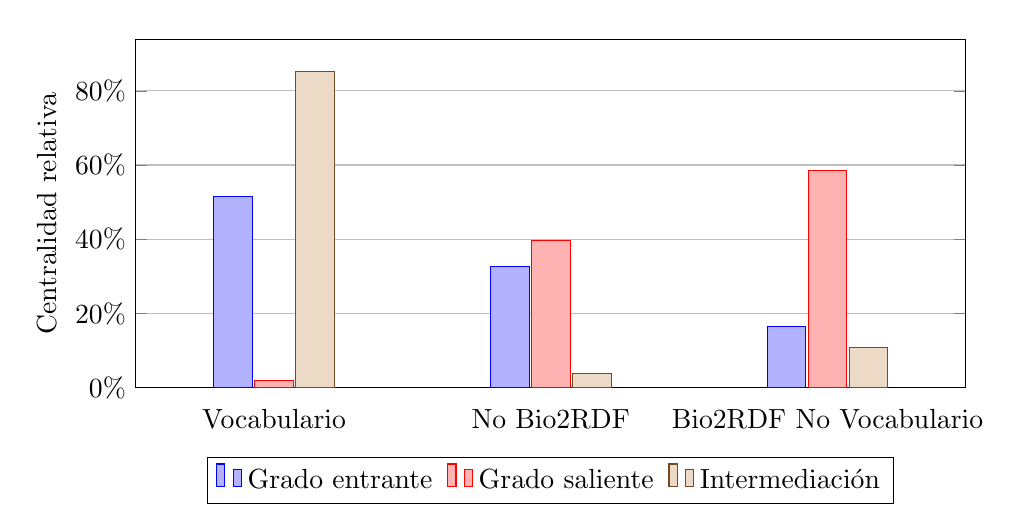
\begin{tikzpicture}
    \begin{axis}[
        width=\textwidth,height = 6cm,
        major x tick style = transparent,
        ybar=2*\pgflinewidth,
        bar width=14pt,
        ymajorgrids = true,
        ylabel = {Centralidad relativa},
        yticklabel={\pgfmathprintnumber{\tick}\%},
        symbolic x coords={Vocabulario,No Bio2RDF,Bio2RDF No Vocabulario},
        xtick = data,
        scaled y ticks = false,
        enlarge x limits=0.25,
        ymin=0,
        legend style={at={(0.5,-0.2)}, anchor=north,legend columns=-1}]
        \addplot coordinates {(Vocabulario, 51.51) (No Bio2RDF, 32.72) (Bio2RDF No Vocabulario, 16.44)};
        \addplot coordinates {(Vocabulario, 1.83)  (No Bio2RDF, 39.62) (Bio2RDF No Vocabulario, 58.54)};
        \addplot coordinates {(Vocabulario, 85.23) (No Bio2RDF, 3.84)  (Bio2RDF No Vocabulario, 10.92)};
        \legend{Grado entrante\,\,, Grado saliente\,\,, Intermediación};
    \end{axis}
  \end{tikzpicture}
  \caption{Centralidad relativa por tipo de dato.}
  \label{fig:comptype}
\end{figure}

\section{Conclusiones}\label{sec:con}
